\documentclass[11pt]{article}
\usepackage{icmlko}
\begin{document}

\title{틀린 위약으로 기각한 것을 되살렸다 --- 만화 재심}
\author{월드모델 실험실}
\date{노트 393 · 2026년 8월 1일}
\maketitle

\begin{abstract}
노트 392가 밝혔다 --- \emph{위약을 어디서 섞느냐가 무엇을 검사하는지
정한다.} 기존 라벨 범위 \textbf{안}의 새 행은 새 것끼리 섞는 위약1이
맞고, \textbf{밖}의 새 행은 옛 학습 행과 맞바꾸는 위약2 라야 한다 ---
위약1은 밖의 행이 나르는 무리 수준 연합을 안 건드리기 때문이다.

\textbf{그러면 노트 389가 틀린 도구로 기각했다.} 만화 바닥 아래 4,999행은
100\%가 범위 밖인데 위약1로 재서 ``잔량 91\% --- 정보가 아니다''로
기각했다. 다시 쟀다.

\begin{center}
\begin{tabular}{lrr}
\hline
 & 위약1 (노트 389) & \textbf{위약2} (옳은 것) \\
\hline
만화 잔량 & 91\% & \textbf{19\%} \\
팝업 잔량 & 99\% & $\mathbf{-25\%}$ \\
\hline
\end{tabular}
\end{center}

\textbf{둘 다 뒤집힌다.} 올바른 위약을 쓰면 만화의 $+0.0952$ 도 배포
도메인의 $+0.0647$ 도 정보다 --- 무리 수준 연합을 깨면 사라지고 심지어
음수로 간다.

규약을 밟았다: 판 $-0.0012$ · 4/12 로 미결정 $\to$ 배포(팝업) $+0.0647$ ·
\textbf{12/12} 로 넣으라 함 $\to$ 조건 ② 열한 도메인 전부 통과(제일 나쁜
모바일이 $|t|{=}2.18$) $\to$ 조항 ⑤ 통과. \textbf{채택한다.}

\textbf{새 챔피언: 판 0.4435 · 분모 3,430 · 만화 학습 5,647.} 만화가
$+0.2487 \to +0.3503$, 팝업이 $+0.4013 \to +0.4872$ 다.

\textbf{교훈은 도구 쪽이다.} 위약이 틀리면 채택도 기각도 다 틀린다 ---
노트 389는 \emph{기각}을 틀렸고 노트 391은 \emph{채택의 이유}를 틀렸다.
같은 하루에 같은 도구로 두 번 틀렸다.
\end{abstract}

\section{되살린 이유}

노트 389는 만화 4,999행을 넣고 위약1(새 행끼리 라벨 섞기)을 붙여
``잔량 91\%''를 얻었다. 그리고 기각했다 --- ``정보가 아니라 라벨 분포가
아래로 이동한 것 자체의 효과다.''

노트 392가 그 해석을 반증했다. 범위 밖 행이 나르는 것은 \emph{무리 수준
연합}(``이런 축을 가진 것들은 라벨이 낮다'')이고, 위약1은 새 행끼리만
섞으므로 그 연합을 그대로 남긴다. \textbf{범위 밖 행에 위약1을 쓰면
아무것도 검사하지 않는다.}

만화의 4,999행은 popularity 420\,--\,632 로 \textbf{100\%가 기존 학습
범위(5,306\,--\,32만) 밖}이다. 그러니 노트 389가 쓴 도구가 그 자료에는
맞지 않았다.

\begin{figure}[t]
\centering
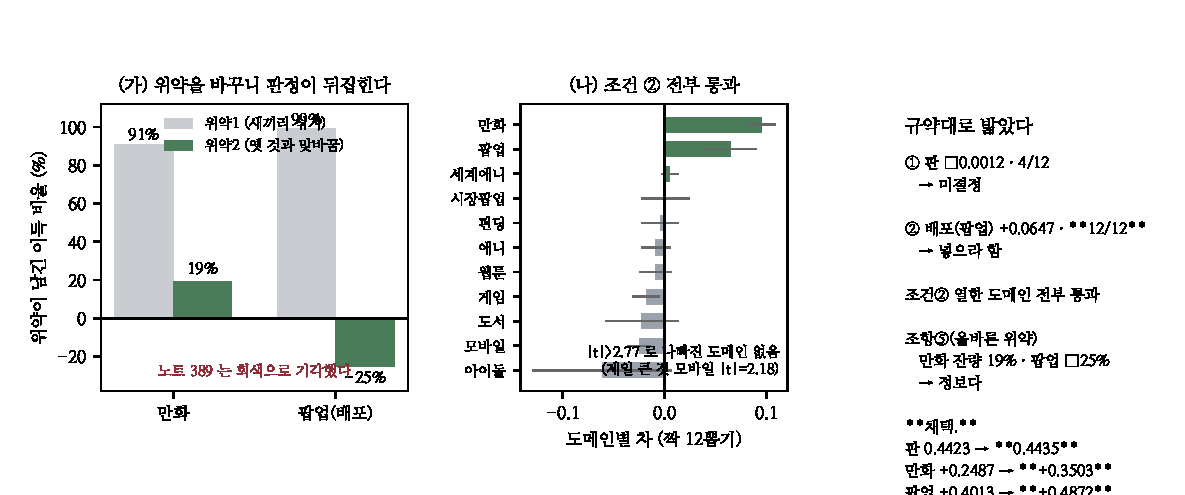
\includegraphics[width=\linewidth]{figs/fig393.pdf}
\caption{\textbf{(가)} 같은 자료를 위약1과 위약2로 재면 잔량이 뒤집힌다.
\textbf{(나)} 도메인별 차와 짝 SD --- 조건 ②에 걸리는 도메인이 없다.
\textbf{(다)} 규약을 밟은 순서.}
\label{fig:main}
\end{figure}

\section{다시 쟀다}

위약2 는 새 행 4,999개의 라벨을 옛 학습 1,783행의 라벨과 맞바꾼다(짝
1,783개, 씨앗 고정). 학습 전체의 라벨 다발은 그대로이고 무리 수준 연합만
거꾸로 실린다.

\begin{center}
\begin{tabular}{lrrl}
\hline
 & 만화 차 & 팝업 차 & 판 차 \\
\hline
B 실제 & $+0.0952$ (12/12) & $+0.0647$ (12/12) & $-0.0012$ (4/12) \\
위약1 (노트 389) & $+0.0864$ (12/12) & $+0.0643$ (12/12) & $-0.0017$ (5/12) \\
\textbf{위약2} & $\mathbf{+0.0185}$ (8/12) & $\mathbf{-0.0159}$ (4/12) & $+0.0001$ (7/12) \\
\hline
\end{tabular}
\end{center}

\textbf{위약2가 만화 이득의 81\%를 지우고 팝업 이득은 통째로 지우고
넘어간다.} 두 이득 다 무리 수준 연합에 실려 있었다 --- 실재하는 정보다.

\section{규약을 밟는다}

\begin{enumerate}
\item \textbf{판} $-0.0012$ · 4/12 --- $|{-}0.0012| < 2\times$짝SD 이고 부호가
4\,--\,8 사이라 \textbf{미결정}(노트 367 · 378 조항 ①).
\item \textbf{배포} 팝업 $+0.0647$ · \textbf{12/12} --- 부호가 9/12 를
넘으므로 배포가 정한다: \textbf{넣는다}(조항 ②).
\item \textbf{조건 ②} 열한 도메인 중 $|t|>2.77$ 로 나빠진 것이 없다. 제일
나쁜 것이 모바일 $-0.0249$(SD 0.0114, $|t|{=}2.18$)이고 그다음이 게임
$-0.0182$($|t|{=}1.34$)다.
\item \textbf{조항 ⑤} 올바른 위약(범위 밖이므로 위약2)으로 만화 잔량
19\% · 팝업 잔량 $-25$\% --- 이득이 정보다.
\end{enumerate}

\textbf{채택.} 만화 학습 $1{,}783 \to 5{,}647$, 판 $0.4423 \to 0.4435$.

\textbf{불편한 자리를 적어 둔다.} 판의 짝 차이가 $-0.0012$(4/12)로 살짝
음수인데 배포가 12/12 로 넣으라 해서 채택됐다. 노트 378이 만든 구조가
그대로 작동한 것이고 --- 판이 못 정하면 배포가 정한다 --- 이번에는 그
배포 신호가 위약2를 통과했으므로 노트 389에서 걱정한 종류의 가짜가
아니다. \textbf{규약을 바꾸고 싶으면 사전 등록하고 관문을 돌린다}(노트
380이 무게 규칙에서 그렇게 했고 못 바꿨다).

\section{도구가 틀리면 양쪽으로 틀린다}

하루 사이에 같은 도구로 두 번 틀렸다.

\begin{center}
\begin{tabular}{lll}
\hline
노트 & 무엇을 틀렸나 & 어느 쪽으로 \\
\hline
389 & 만화를 기각했다 & \textbf{거짓 음성} \\
391 & 펀딩 밖 행을 ``눈금''이라 했다 & \textbf{거짓 해석} \\
\hline
\end{tabular}
\end{center}

\textbf{위약은 ``무엇을 지우는가''로 고른다.} 검사하려는 정보가 그 위약이
안 지우는 자리에 있으면 그 검사는 통과도 탈락도 뜻이 없다. 조항 ⑤에
그 문장을 붙인다.

\section{남은 것}

\begin{center}
\begin{tabular}{lll}
\hline
항목 & 왜 값이 큰가 & 어떻게 \\
\hline
웹툰 835 안/밖 분해 & 아직 안 갈랐다 & 안은 위약1 · 밖은 위약2 \\
애니 아카이브 & 무게 606 · 덮음 22\% & 수집 중(900/3,000) \\
만화 더 아래 & 420 아래가 아직 있다 & popularity\_lesser 를 더 내린다 \\
무리 수준 정보의 상한 & 판이 그것을 다 못 볼 수 있다 & 무리 표시자로 잰다 \\
\hline
\end{tabular}
\end{center}

\end{document}
